\section{Summary of Paper \ref{pap:pit}}
\subsection*{"\nameref{pap:pit}"}
\subsection*{Scope and motivations}
In order to expand the modeling complexity and uncertainty from Paper \ref{pap:rolldamping}, system identification of manoeuvring by adding the the surge, sway, and yaw degrees of freedom was studied in Paper \ref{pap:pit}. 
The objective was to find parametric model structures with good generalization and to develop parameter identification techniques  from FRMT data.

The dynamics were assumed to be described by an Abkowitz or truncated Abkowitz model. 
The system identification method proposed in Paper \ref{pap:pit} was validated on two case study ships: the wPCC (\autoref{fig:wpcc-mdl}) and the KVLCC2 (\autoref{fig:kvlcc2_hsva}). The parameters were identified with the recursive inverse dynamics regression (see \autoref{sec:RIDR}) and the model structures were developed using the process described in \autoref{sec:cross_validation}. Consequently, both test cases aimed to predict turning circle maneuvers. 

\begin{figure}[h!]
\centering
\includegraphics[width=0.7\linewidth]{kappa/images/wpcc_mdl.png}
\caption{wPCC tested at SSPA Maritime center. Copyright 2020 by RISE.}
\label{fig:wpcc-mdl}
\end{figure}

\begin{figure}[h!]
    \centering
    \begin{subfigure}[b]{0.45\textwidth}
    \centering
    \includegraphics[height=3cm]{kappa/images/kvlcc2_front.png}
    \end{subfigure}
    ~
     \begin{subfigure}[b]{0.45\textwidth}
     \centering
     \includegraphics[height=3cm]{kappa/images/kvlcc2_aft.png}
     \end{subfigure}
    \caption{Ship model used in HSVA and MARIN model tests. Copyright HSVA.}
    \label{fig:kvlcc2_hsva}
\end{figure}


\subsection*{Results and concluding remarks}
The wPCC test case focuses on predicting forces and moments from the ship hull and the rudders. The propeller force is not part of the prediction model; it is obtained from the model test measurements.
In the model development process (\autoref{sec:cross_validation}), the model test data used for modelling is split into the training test, the validation test, and the test data sets (also presented in \autoref{fig:wpcc_datasets}), 
\vspace{5pt}
\begin{itemize}
    \setlength\itemsep{5pt}
    \item The training dataset: self-propulsion, pull-out tests, and zigzag10/10 tests to starboard and port.
    \item The validation dataset: three zigzag20/20 tests.
    \item Test dataset: one turning circle test.
\end{itemize}
\begin{figure}[h!]
\centering
\includegraphics[width= 1.0\linewidth]{kappa/images/3.pdf}
\caption{wPCC training, validation and testing datasets.}
\label{fig:wpcc_datasets}
\end{figure}
\noindent If the manoeuvring model built by the proposed method based on a series of model tests (including ZigZag10/10 and 20/20 to port and starboard as well as the self-propulsion and pull out test) \cite{imoStandardsShipManoeuvrability2002} can predict the turning circle maneuver, then it is a capable model. The linear model (LVMM) was ruled too simple for the wPCC. Only the AVMM and MAVMM were considered possible manoeuvring models in the model selection.
Forces and moment predicted for the validation dataset, with the manoeuvring models fitted with proposed parameter estimation on the training set, are presented in \autoref{fig:validation-forces}. The fitted AVMM over-predicts the forces by far. 
\begin{figure}[h!]
\centering
\includegraphics[width=1.0\textwidth]{kappa/images/7.pdf}
\caption{Validation of force models for wPCC ZigZag20/20.}\label{fig:validation-forces}
\end{figure}
\noindent The over-prediction of forces with the AVMM can be explained by the major problems with multicollinearity (see \autoref{sec:multicollinearity}) that were encountered when applying the parameter estimation method to the wPCC data.
\begin{figure}[ht!]
\centering
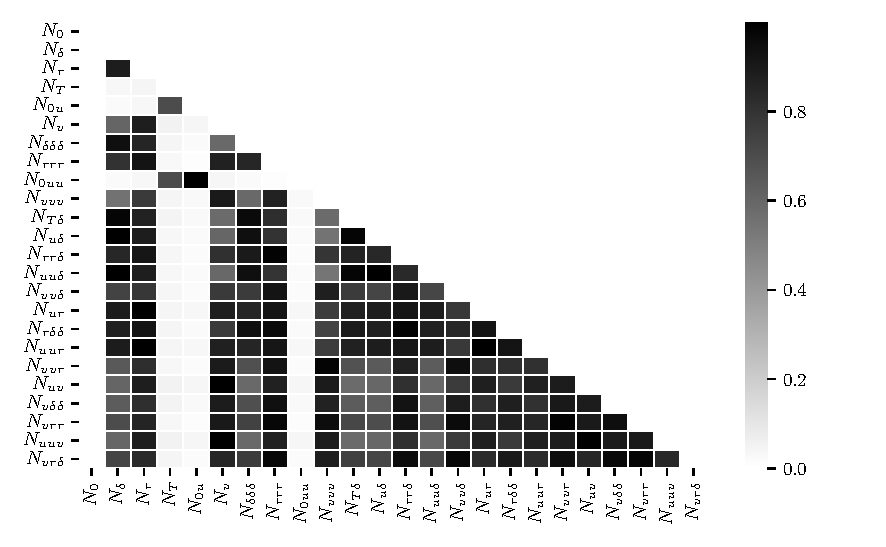
\includegraphics[width=1.0\textwidth]{kappa/images/10.pdf}
\caption{Absolute correlation between the features in the wPCC yaw moment regression of AVMM.}\label{\detokenize{06.10_results_wpcc:fig-ncorr}}
\end{figure}
\clearpage
The absolute correlation coefficient between the features in the wPCC yaw moment regression is presented in \hyperref[\detokenize{06.10_results_wpcc:fig-ncorr}]{\autoref{\detokenize{06.10_results_wpcc:fig-ncorr}}}. Most of the coefficients have a very high absolute correlation (indicated in black). Some of the regressed hydrodynamic derivatives in the AVMM also have substantial values and large degrees of uncertainty. Therefore, simulations of the validation cases are only possible using the MAVMM. The simulations are displayed for one of the ZigZag20/20 validation cases in \hyperref[\detokenize{06.10_results_wpcc:fig-validation-sim}]{\autoref{\detokenize{06.10_results_wpcc:fig-validation-sim}}}.
\begin{figure}[h!]
\centering
\includegraphics[width=1.0\textwidth]{kappa/images/9.pdf}
\caption{Validation with simulations for wPCC ZigZag20/20.}\label{\detokenize{06.10_results_wpcc:fig-validation-sim}}\end{figure}
The MAVMM was therefore selected as the most appropriate model for the wPCC in the validation step of the model development process. This model was retrained on the joined test and validation data set to obtain the final prediction model which was used to predict the turning circle test data set. Advance and tactical diameter \cite{imoStandardsShipManoeuvrability2002} from the prediction differs by 4\% and 1\% from the model test data, as seen in \autoref{\detokenize{06.10_results_wpcc:tab-wpcc-advance}}.
\input{kappa/table_wpcc_turning}
Results from the turning circle prediction are also presented in  \autoref{\detokenize{06.10_results_wpcc:fig-track-plot-testing-sim}} and  \autoref{\detokenize{06.10_results_wpcc:fig-testing-sim}}. Monte Carlo simulations with alternative realizations of the regression, considering the uncertainty in the regressed parameters, are also displayed in these figures. The alternative realizations have similar simulation results to the model with mean values of the regression (black line).
\begin{figure}[ht]
\centering
\includegraphics[width=0.90\textwidth]{kappa/images/11.pdf}
\caption{Turning circle test case for wPCC, track plots from model test and simulation.}\label{\detokenize{06.10_results_wpcc:fig-track-plot-testing-sim}}\end{figure}
\begin{figure}[ht!]
\centering
\includegraphics[width=0.90\textwidth]{kappa/images/12.pdf}
\caption{Turning circle test case for wPCC, time series from model test and simulation.}\label{\detokenize{06.10_results_wpcc:fig-testing-sim}}\end{figure}
\clearpage
\noindent The mean values and standard error (se) of the hydrodynamic derivatives (expressed with prime units for the wPCC) obtained with parameter estimation of MAVMM (\autoref{equation:02.01_manoeuvring models:eqxmartinssimple}, \autoref{equation:02.01_manoeuvring models:eqymartinssimple},  \autoref{equation:02.01_manoeuvring models:eqnmartinssimple}) applied to all the wPCC data (including the turning circle)  are displayed in \hyperref[\detokenize{06.10_results_wpcc:wpcc-derivatives}]{Table \ref{\detokenize{06.10_results_wpcc:wpcc-derivatives}}}.
\input{kappa/table_wpcc_derivatives}
\clearpage
\subsection{The KVLCC2 test case}
\label{\detokenize{05.01_case_studies:the-kvlcc2-test-scenarios}}
The proposed system identification method is also validated using the KVLCC2 case study ship model.
The propeller is in the manoeuvring model for this test case (instead of only the hull and rudders, as in the wPCC test case) so that the entire ship can be simulated without additional input.
The model development process, which is described in \autoref{sec:cross_validation}, is applied to the KVLCC2 as well.
The data has been split into training, validation, and test data sets (also seen in \autoref{fig:kvlcc2_datasets}),
\vspace{5pt}
\begin{itemize}
    \setlength\itemsep{5pt}
    \item Training dataset: various zigzag tests to starboard and port from model tests carried out at HSVA for the SIMMAN2008 conference \cite{sternExperienceSIMMAN20082011}.
    \item Validation dataset: ZigZag35/5 carried out at HSVA for the SIMMAN2008 conference \cite{sternExperienceSIMMAN20082011}.
    \item Test dataset: turning circle model tests carried out at MARIN for the SIMMAN2008 conference \cite{sternExperienceSIMMAN20082011}
\end{itemize}
\vspace{5pt}
\noindent A propeller prediction model is needed for the KVLCC2, which is developed from thrust measurements from the model tests, as described in the next section.
\begin{figure}[h!]
\centering
\includegraphics[width=1.0\textwidth]{kappa/images/4.pdf}
\caption{KVLCC2 training, validation and testing datasets.}\label{fig:kvlcc2_datasets}\end{figure}
\subsubsection{The KVLCC2 propeller model}
\label{\detokenize{06.20_results_kvlcc2:the-kvlcc2-propeller-model}}\label{\detokenize{06.20_results_kvlcc2:results-propeller-model}}

In the development of a propeller model, the coefficients in the \(K_T\) polynomial (\autoref{equation:02.10_propeller_model:eqkt}) were regressed from the KVLCC2 propeller characteristics from SIMMAN2008 HSVA model tests \cite{sternExperienceSIMMAN20082011}, as seen in \autoref{tab:kt_coefficients}. The propeller model was developed with cross-validation on the training and validation datasets to make the appropriate feature selection.
The cross-validation study was carried out on the three candidate propeller models: 
\vspace{5pt}
\begin{itemize}
    \setlength\itemsep{5pt}
    \item the MMG propeller model
    \item the simple propeller model
    \item the polynomial propeller model
\end{itemize}
\vspace{5pt}
The training and validation sets were derived from the entire model test time series from the HSVA model tests. The model tests were randomly divided into the test and validation sets. The random training and validation sets were repeated 100 times. The Polynomial model was selected due to it having the highest accuracy. Taylor wake \(w_{p0}\) = {0.4} was used in all three models. The MMG model used \(C_1\)={2.0}, \(C_2\)={1.6} when \(\beta_p>0\) and \(C_2\)={1.1} when \(\beta_p<=0\) \cite{yasukawaIntroductionMMGStandard2015}. \hyperref[\detokenize{06.20_results_kvlcc2:fig-propeller-validation}]{\autoref{\detokenize{06.20_results_kvlcc2:fig-propeller-validation}}} displays a small portion of the cross-validation. Coefficients of the polynomial propeller model fitted on the training and validation datasets for KVLCC2 are presented in \hyperref[\detokenize{06.20_results_kvlcc2:kvlcc2-propeller-model}]{Table \ref{\detokenize{06.20_results_kvlcc2:kvlcc2-propeller-model}}}.

\vspace{0.2cm}
\begin{minipage}[c]{0.49\textwidth}
    \vspace{-0.40cm}
    \centering
    \captionof{table}{\(K_T\) polynomial coefficients.}
    \label{tab:kt_coefficients}
    \begin{tabular}{c c}
        \toprule
        Coefficient & Value \\
        \hline
        k_0 & 0.32419 \\
        k_1 & -0.22091 \\
        k_2 & -0.14905 \\
        \bottomrule
    \end{tabular}
%\end{table}
\end{minipage}
\hfill
\begin{minipage}[c]{0.49\textwidth}
\captionof{table}{KVLCC2 propeller model.}
\label{\detokenize{06.20_results_kvlcc2:kvlcc2-propeller-model}}
%\begin{table}[h]
%    \centering
%        \caption{KVLCC2 propeller model.}
%    \label{\detokenize{06.20_results_kvlcc2:kvlcc2-propeller-model}}
    \begin{tabular}{l l l}
\toprule
 & 

\(\beta_p>0\)
& 

\(\beta_p<=0\)
\\
\hline

\(C_1\)
&

-0.1735
&

-0.1066
\\


\(C_2\)
&

0.4589
&

0.0771
\\


\(C_3\)
&

-1.8865
&

1.2958
\\


\(C_4\)
&

0.0515
&

0.0514
\\
\bottomrule
\end{tabular}

%\end{table}


\end{minipage}
\vspace{-0.5cm}
\begin{figure}[!htb]
\centering
\includegraphics[width=0.69\textwidth]{kappa/images/13.pdf}
\caption{Validation of MMG, Simple, and Polynomial propeller models for KVLCC2.}\label{\detokenize{06.20_results_kvlcc2:fig-propeller-validation}}\end{figure}
\clearpage
\subsubsection{KVLCC2 manoeuvring model}
\label{\detokenize{06.20_results_kvlcc2:kvlcc2-manoeuvring-model}}
The linear manoeuvring model (LVMM) was ruled too simple for KVLCC2. Only the AVMM and MAVMM were considered possible manoeuvring models in the model selection.
The forces and moments applied on the hull, rudder, and propeller predicted with the AVMM and MAVMM fitted with the proposed parameter estimation on the training set are displayed in \hyperref[\detokenize{06.20_results_kvlcc2:fig-kvlcc2-validation-forces}]{\autoref{\detokenize{06.20_results_kvlcc2:fig-kvlcc2-validation-forces}}}.
The forces are accurately predicted with both manoeuvring models. The AVMM does not provide the large over-predictions that were observed from wPCC. However, the MAVMM is still slightly better and is therefore selected as the suitable manoeuvring model for the KVLCC2.
Simulations of the validation cases with the MAVMM are displayed for one of the ZigZag20/20 validation cases in \hyperref[\detokenize{06.20_results_kvlcc2:fig-kvlcc2-validation-sim}]{\autoref{\detokenize{06.20_results_kvlcc2:fig-kvlcc2-validation-sim}}} and \hyperref[\detokenize{06.20_results_kvlcc2:fig-kvlcc2-validation-sim-error}]{\autoref{\detokenize{06.20_results_kvlcc2:fig-kvlcc2-validation-sim-error}}}, where the predicted thrust is also shown.
\begin{figure}[h]
\centering
\includegraphics[width=1.0\textwidth]{kappa/images/14.pdf}
\caption{Validation of force models for KVLCC2.}\label{\detokenize{06.20_results_kvlcc2:fig-kvlcc2-validation-forces}}\end{figure}
\begin{figure}[h]
\centering
\includegraphics[width=1.0\textwidth]{kappa/images/15.pdf}
\caption{Validation with simulations for KVLCC2.}\label{\detokenize{06.20_results_kvlcc2:fig-kvlcc2-validation-sim}}\end{figure}
\begin{figure}[h]
\centering
\includegraphics[width=1.0\textwidth]{kappa/images/16.pdf}
\caption{Validation error (prediction minus (-) model test) with simulations for KVLCC2.}\label{\detokenize{06.20_results_kvlcc2:fig-kvlcc2-validation-sim-error}}\end{figure}
\clearpage
\noindent Results from the final prediction of the turning circle test are shown in  \hyperref[\detokenize{06.20_results_kvlcc2:fig-kvlcc2-track-plot-testing-sim}]{\autoref{\detokenize{06.20_results_kvlcc2:fig-kvlcc2-track-plot-testing-sim}}}, \hyperref[\detokenize{06.20_results_kvlcc2:fig-kvlcc2-testing-sim}]{\autoref{\detokenize{06.20_results_kvlcc2:fig-kvlcc2-testing-sim}}} and \hyperref[\detokenize{06.20_results_kvlcc2:fig-kvlcc2-testing-sim-error}]{\autoref{\detokenize{06.20_results_kvlcc2:fig-kvlcc2-testing-sim-error}}}. The prediction is conducted using simulation with the MAVMM trained on the training and validation datasets. Monte Carlo simulations with alternative realizations of the regression are also displayed in this figure. The alternative realizations are very similar to the model with mean values of the regression (black line).
\begin{figure}[h!]
\centering
\includegraphics[width=1.0\textwidth]{kappa/images/17.pdf}
\caption{Comparison between the predicted turning circle test with MAVMM trained on HSVA data and MARIN model test results for KVLCC2.}\label{\detokenize{06.20_results_kvlcc2:fig-kvlcc2-track-plot-testing-sim}}\end{figure}
\begin{figure}[h!]
\centering
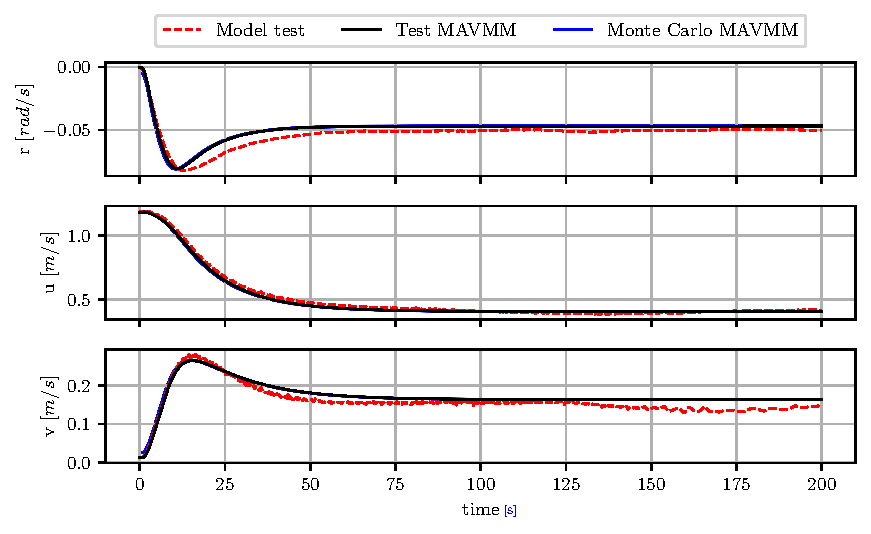
\includegraphics[width=1.0\textwidth]{kappa/images/18.pdf}
\caption{Comparison between the predicted turning circle test with MAVMM trained on HSVA data and MARIN model test results for KVLCC2.}\label{\detokenize{06.20_results_kvlcc2:fig-kvlcc2-testing-sim}}\end{figure}
\begin{figure}[h!]
\centering
\includegraphics[width=1.0\textwidth]{kappa/images/19.pdf}
\caption{The prediction error (prediction minus (-) model test) for the turning circle test with MAVMM trained on HSVA data and MARIN model test results for KVLCC2.}\label{\detokenize{06.20_results_kvlcc2:fig-kvlcc2-testing-sim-error}}\end{figure} 

Comparisons of turning circle advance and tactical diameters compared to the model test results are displayed in \hyperref[\detokenize{06.20_results_kvlcc2:tab-kvlcc2-advance}]{Table \ref{\detokenize{06.20_results_kvlcc2:tab-kvlcc2-advance}}}. Predicted advance and tactical diameters differ by 2\% and 5\%, which is considered acceptable because of the margin of the IMO standard limits (which are also displayed in this table). The results are also closer to the model tests than a similar study conducted for the KVLCC2 \cite{heNonparametricModelingShip2022}.
\renewcommand{\cellalign}{vh}
\renewcommand{\theadalign}{vh}
\begin{table}[h]
    \centering
    \footnotesize
        \caption{KVLCC2 Predicted turning circle advance (A) and tactical diameter (TD) compared to MARIN model tests and IMO limit.}
    \label{\detokenize{06.20_results_kvlcc2:tab-kvlcc2-advance}}
    \begin{tabular}{p{0.7cm} p{1.5cm} p{1.3cm} p{1.0cm} p{1.3cm} p{1.3cm} p{1.0cm} }
\toprule
 

$\delta$
& 

\thead{A \\ (model test) \\ {[}m{]}}
& 

\thead{A \\ (prediction) \\ {[}m{]}}
& 

\thead{A \\ (IMO) \\ {[}m{]}}
& 

\thead{TD \\ (model test) \\ {[}m{]}}
& 

\thead{TD \\ (prediction) \\ {[}m{]}}
& 

\thead{TD \\ (IMO) \\ {[}m{]}}
\\
\hline

35.0
&

21.59
&

21.21
&

31.5
&

21.72
&

23.07
&

35.0
\\


-35.0
&

22.54
&

22.1
&

31.5
&

23.55
&

24.29
&

35.0
\\
\bottomrule
\end{tabular}
\end{table}

\clearpage
The mean values and standard error (se) of the hydrodynamic derivatives (expressed with prime units for the KVLCC2) obtained with parameter estimation of MAVMM (\autoref{equation:02.01_manoeuvring models:eqxmartinssimple}, \autoref{equation:02.01_manoeuvring models:eqymartinssimple}, \autoref{equation:02.01_manoeuvring models:eqnmartinssimple}) applied on all the HSVA data are shown in \hyperref[\detokenize{06.20_results_kvlcc2:kvlcc2-derivatives}]{Table \ref{\detokenize{06.20_results_kvlcc2:kvlcc2-derivatives}}}.
\input{kappa/table_kvlcc2_derivatives}
\section*{}
\vspace{-1cm}
\subsection{Inverse dynamics}
\label{\detokenize{06.40_results_inverse_dynamics:inverse-dynamics}}\label{\detokenize{06.40_results_inverse_dynamics::doc}}
The capability of the inverse dynamics on simulated data was also investigated in Paper \ref{pap:pit}. The hydrodynamic derivatives within the manoeuvring model can be identified exactly at ideal conditions for the parameter estimation with no measurement noise and a perfect estimator. For example, artificial data from a turning circle test can be simulated by a predefined/true manoeuvring model. The hydrodynamic derivatives within the manoeuvring model can be identified with the same values. Results from such a simulation are presented in \hyperref[\detokenize{06.40_results_inverse_dynamics:fig-bar-parameters}]{\autoref{\detokenize{06.40_results_inverse_dynamics:fig-bar-parameters}}}, where the regression has identified the true values precisely.
\begin{figure}[h!]
\centering
\includegraphics[width=\linewidth]{kappa/images/5.pdf}
\caption{True and regressed hydrodynamic derivatives in MAVMM identified with Inverse dynamics and OLS regression on a simulated turning circle with MAVMM.}\label{\detokenize{06.40_results_inverse_dynamics:fig-bar-parameters}}\end{figure}


\subsection{Preprocessing}
\label{\detokenize{06.31_results_noise:preprocessing}}\label{\detokenize{06.31_results_noise::doc}}

The low-pass filter is a prevalent alternative to preprocessing the model test data, as opposed to the EKF used by the proposed parameter estimation.
In order to investigate which filter is the most effective, the proposed parameter estimation was run on the wPCC model test data with the EKF + RTS smoother replaced with a low-pass filter. The low-pass filter applies a first-order linear digital Butterworth filter twice (once forward and once backward) for zero-phase conditions \cite{virtanenSciPy10Fundamental2020}. \hyperref[\detokenize{06.31_results_noise:fig-lowpass-accuracy}]{\autoref{\detokenize{06.31_results_noise:fig-lowpass-accuracy}}} displays the average simulation error \( \overline{RMSE} \) with low-pass filters at various cutoff frequencies for all wPCC model tests. Corresponding error with parameter estimation using EKF + RTS is also presented in the figure. The simulation error for each model test is expressed as the root mean square error \(RMSE\) (\autoref{equation:06.31_results_noise:eqrmse}) of the distance between the position from the model test and simulation.
\begin{equation}\label{equation:06.31_results_noise:eqrmse}
\begin{split}RMSE=\sqrt{ \frac{\sum_{n=1}^{N} (d_n^2) }{N}} \end{split}
\end{equation}
where \(d_n\) is the euclidean distance for each time step between the model test positions (\(x_0\), \(y_0\)) and the predicted positions.
\begin{figure}[h!]
\centering
\includegraphics[width=1.0\textwidth]{kappa/images/6.pdf}
\caption{Average simulation error with MAVMM fitted on wPCC model test data using low-pass filters with various cutoff frequencies or EKF.}\label{\detokenize{06.31_results_noise:fig-lowpass-accuracy}}\end{figure} 
\noindent The simulations show that high accuracy can be obtained using a low-pass filter as the preprocessor if an optimal cutoff frequency is selected. The low-pass filter's accuracy decreases quickly at lower or higher frequencies. Higher cutoff frequencies result in too much measurement error in the data, which causes the OLS regression to perform poorly. In extreme cases, it is similar to having no filter. An extremely low cutoff frequency removes too much, including parts of the actual signal. The results show that the low-pass filter with a 7 Hz cutoff frequency has the lowest error rate among the low-pass filters. The EKF + RTS method in the parameter estimation has an even lower error rate, which is why it is used as the preprocessor in the proposed parameter estimation.

\textcolor{red}{
It was proposed to run the two-step method \cite{yoonIdentificationHydrodynamicCoefficients2003} iteratively.    
In the first step of the two-step method, velocities and accelerations were estimated using an EKF with a manoeuvring model as predictor. In the second step, the inverse dynamics regression was applied to the EKF estimated states.
}